\chapter{Wprowadzenie}
\label{cha:wprowadzenie}

%---------------------------------------------------------------------------

\section{Cel pracy}
\label{sec:celPracy}

Celem pracy jest zaprojektowanie, implementacja i ewaluacja mechanizmu pozyskiwania wiedzy o stanie emocjonalnym użytkownika w systemach \textit{affective computing}. W szczególności w ramach pracy przeprowadzona zostanie analiza istniejących rozwiązań, na bazie którego opracowane zostanie rozwiązanie pozwalające na odpytywanie użytkownika o stan emocjonalny w sposób nieintruzywny.

%---------------------------------------------------------------------------

\section{Zastosowania wykrywania emocji}
\label{sec:zastosowaniaWykrywaniaEmocji}

Wyobraźmy sobie świat, w którym maszyna potrafi rozpoznawać emocje. Po ciężkim dniu wchodzimy do domu, a z zestawu stereo wybrzmiewa już muzyka adekwatna do naszego nastroju. Uruchamiamy grę wideo, a jej algorytm potrafi rozpoznać, jak reagujemy na kolejne wyzwania. Chcemy poszerzyć horyzonty -– inteligentny system e-learningowy prowadzi nas w dokładnie takim tempie, jakiego potrzebujemy. Kiedy jesteśmy przybici jesienną aurą, strona, która wyświetla nam reklamę, nie proponuje zakupu trampoliny, ale ciepłe bambosze USB. A gdy, nie daj Boże, przytrafia nam się nieszczęście, system awaryjny wzywa pomoc, której udaje się zdążyć na czas.

Ale w jaki sposób mamy przekazywać swoje emocje do aplikacji? Komputer ma mikrofon, klawiaturę i myszkę, które można wykorzystywać do przekazywania mu informacji. Problem w tym, że nie zawsze jesteśmy przy komputerze i że nie zawsze wystarczy mikrofon, klawiatura i myszka. Na szczęście jest urządzenie, które współczesny człowiek ma niemal zawsze przy sobie –- telefon komórkowy.


%---------------------------------------------------------------------------

\section{Gromadzenie danych}
\label{sec:gromadzenieDanych}

Niestety jego możliwości poznawcze są ograniczone. Telefon potrafi odczytać położenie za pomocą żyroskopu, czy tekst za pomocą dotykowej klawiatury. Idea \textit{HowAreYou} polega na tym, żeby te ograniczone sygnały połączyć i za ich pomocą odczytać nastrój użytkownika. Smartfon może też zrobić zdjęcie kamerą -- za pomocą fotografii już teraz można całkiem dokładnie określić nastrój użytkownika. Można też wprost zapytać użytkownika telefonu –- jeżeli nie nadużyjemy tego rozwiązania, stwarza ono szeroki wachlarz możliwości.

Celem HowAreYou jest zbieranie dużej ilości danych -- zarówno zrozumiałych (czyli takich, które system potrafi odczytać), jak i niezrozumiałych. Dzięki bazie, która może powstać w przyszłości, przyszłe aplikacje będą mogły bezinwazyjnie odczytywać nastrój użytkownika.

\begin{figure}[H]
	\centering
	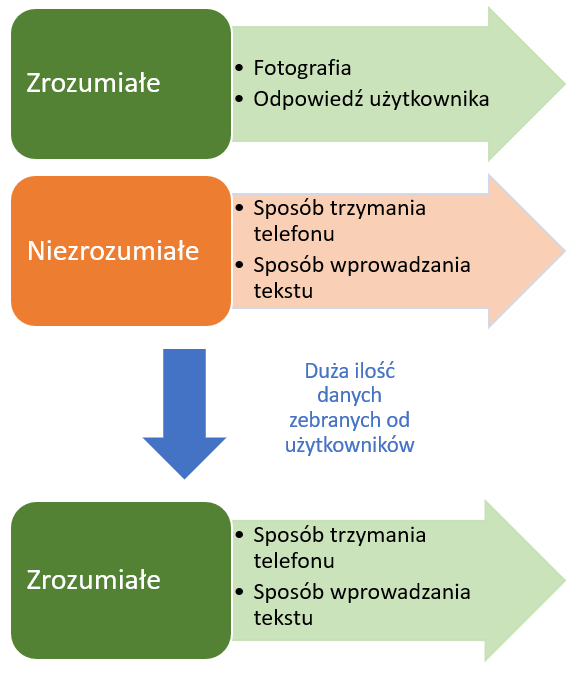
\includegraphics[scale=0.7]{rozdzial1/gromadzenieDanych.png}
	\caption{Schemat przedstawia jak \textit{HowAreYou} lub podobna aplikacja może wpłynąć na uczynienie niezrozumiałych obecnie czynników zrozumiałymi. W niniejszym badaniu nie został uwzględniony sposób wprowadzania tekstu. Podano go tutaj jako jedną z możliwości rozwinięcia pluginu \textit{HowAreYou} w przyszłości.}
\end{figure}

Projektowanie tej aplikacji jest zadaniem niezwykle delikatnym. Człowiek, co naturalne, lubi strzec swojej prywatności. Zrezygnuje, jeżeli będzie nieustannie niepokojony, albo poczuje, że traci kontrolę nad danymi, które trafiają do bazy. Konieczne jest zaprojektowanie takiego systemu, który da użytkownikowi możliwość wyboru i pewność, że treści, które udostępnia, są przez niego kontrolowane i całkowicie bezpieczne.